\documentclass[conference]{IEEEtran}
\IEEEoverridecommandlockouts

\usepackage[T1]{fontenc}
\usepackage{cite}
\usepackage{amsmath,amssymb,amsfonts}
\usepackage{graphicx}
\usepackage{booktabs}
\usepackage{multirow}
\usepackage{textcomp}
\usepackage{xcolor}
\usepackage{tikz}
\usetikzlibrary{positioning,arrows.meta,calc}
\usepackage[hidelinks]{hyperref}

\graphicspath{{figures/}}
\newcommand{\fu}{Fu~\emph{et~al.}}
\DeclareMathOperator*{\med}{med}

\begin{document}

\title{Kinect Lite: Depth Denoising and Its Effect on\\ Depth-Only ICP Camera Tracking}

\author{%
\IEEEauthorblockN{Keshav Thakur, Nandaa Ramasamy, Nithin N, and Tapan Kumar Pallati}
\IEEEauthorblockA{\rule{0pt}{18pt}\textit{Under the guidance of} Prof.~Krishnan CMC\\[2pt]
Department of Electrical and Electronics Engineering\\
National Institute of Technology Karnataka, Surathkal, India}
}


\maketitle

% ===========================================================================
\noindent\textbf{\textit{Abstract:}} Depth maps from Kinect-style sensors contain spikes
(pixels with a grossly wrong depth) and holes (pixels with no depth). They are usually denoised before
camera tracking with the iterative closest point (ICP) algorithm, on the
assumption that a more accurate depth map gives a more accurate camera path. We
test this assumption by comparing a $9\times9$ median filter with the
spatio-temporal denoiser of \fu{} on the ICL-NUIM and TUM RGB-D datasets. The
median halves the per-pixel depth error (39.2 to 18.8\,mm), while \fu{} barely
changes it (37.7\,mm). For depth-only ICP the ranking reverses: \fu{} reaches a
trajectory error of 0.95\,cm on ICL-NUIM and 3.33\,cm on TUM, against
14.94\,cm and 13.32\,cm for the median. The result holds for every ICP variant
tested and is not changed by hole filling. ICP aligns consecutive frames with
each other, and the median leaves them inconsistent and biased, while \fu{}
makes them agree. A denoiser for tracking should therefore be judged by the
tracking error, not the depth error.

\vspace{0.5\baselineskip}
\noindent\textbf{\textit{Index Terms:}} Depth denoising, Kinect, RGB-D,
iterative closest point, visual odometry, median filter.
\vspace{0.3\baselineskip}

% ===========================================================================
\section{Introduction}

Depth cameras such as the Microsoft Kinect and the Asus Xtion are cheap and
widely used in robotics and 3D scanning. Systems such as
KinectFusion~\cite{newcombe2011kinectfusion} track the camera from depth alone
using the iterative closest point (ICP) algorithm~\cite{besl1992method,chen1992object},
which aligns the point clouds of consecutive frames. Errors in the depth go
straight into the motion estimate and add up over time as drift. ICP works in a loop: it pairs every point of one cloud with its nearest point
in the other, solves for the rotation and translation that best align the
pairs, applies them, and repeats until the fit stops improving. Chaining the
motions of all consecutive frames gives the camera path.

Raw depth has two kinds of error. \emph{Spikes} are
pixels with a grossly wrong depth. \emph{Holes} are pixels with no depth at
all. The usual fix is to denoise the depth before tracking, and denoisers are
usually compared by their per-pixel error against the true depth. The hidden
assumption is that a better depth map gives a better camera path. We test
that assumption.

We compare two denoisers that represent the two common approaches:
\begin{itemize}
\item a $9\times9$ median filter that works on one frame at a time
      (under a minute for 450 frames), and
\item the method of \fu{}~\cite{fu2012kinect}, which fills holes from
      neighbouring frames and smooths over space and time (about 26 minutes
      for 450 frames in our implementation).
\end{itemize}
Both feed the same depth-only ICP tracker. Our findings are:
\begin{enumerate}
\item The median is the better denoiser by depth error, but \fu{} is 4 to 16
      times better for tracking. The two criteria rank them in opposite order.
\item This holds for every ICP variant that ran, and filling the remaining
      holes does not change it.
\item Normals and frame-to-frame agreement explain it: the median leaves
      consecutive frames inconsistent and biased, which ICP reads as motion.
\end{enumerate}

% ===========================================================================
\section{Related Work}

\emph{Depth denoising.} The median filter~\cite{huang1979fast} is the standard
filter for impulsive noise. The bilateral filter~\cite{tomasi1998bilateral}
averages neighbours that are close in both position and depth, so it keeps
edges sharp. \fu{}~\cite{fu2012kinect} designed a method for Kinect-like
sensors that predicts hole values from motion-compensated neighbouring frames
and then applies a spatio-temporal bilateral filter whose strength grows with
depth, following Kinect noise models~\cite{khoshelham2012accuracy,nguyen2012modeling}.

\emph{ICP.} Point-to-point ICP~\cite{besl1992method} minimises distances
between matched points. Point-to-plane ICP~\cite{chen1992object} minimises
distances along the surface normal and usually converges faster and more
accurately~\cite{rusinkiewicz2001efficient}. Generalized ICP
(GICP)~\cite{segal2009generalized} models each point with a local covariance.
We use the Open3D implementations~\cite{zhou2018open3d}.

\emph{Benchmarks.} ICL-NUIM~\cite{handa2014benchmark} is synthetic and has
both the true depth and the true camera path. TUM RGB-D~\cite{sturm2012benchmark}
is real sensor data with a motion-capture camera path but no true depth.

% ===========================================================================
\section{Method}\label{sec:method}

\begin{figure}[!t]
\centering
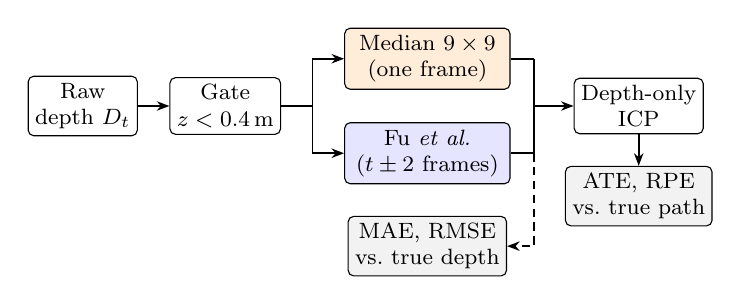
\begin{tikzpicture}[
  font=\footnotesize,
  box/.style={draw, rounded corners=2pt, align=center, minimum height=7mm, inner sep=2.5pt},
  den/.style={box, minimum width=21mm},
  arr/.style={-{Stealth[length=1.6mm]}, semithick},
  node distance=3.5mm and 4mm]
  \node[box] (raw) {Raw\\depth $D_t$};
  \node[box, right=of raw] (gate) {Gate\\$z<0.4$\,m};
  \node[den, right=8mm of gate, yshift=6mm, fill=orange!15] (med) {Median $9\times9$\\(one frame)};
  \node[den, right=8mm of gate, yshift=-6mm, fill=blue!10] (fu) {\fu{}\\($t\pm2$ frames)};
  \node[box, right=8mm of med, yshift=-6mm] (icp) {Depth-only\\ICP};
  \node[box, below=4mm of icp, fill=black!5] (traj) {ATE, RPE\\vs.\ true path};
  \node[box, below=4mm of fu, fill=black!5] (derr) {MAE, RMSE\\vs.\ true depth};
  \draw[arr] (raw) -- (gate);
  \draw[arr] (gate.east) -- ++(4mm,0) |- (med.west);
  \draw[arr] (gate.east) -- ++(4mm,0) |- (fu.west);
  \draw[semithick] (med.east) -- ++(3mm,0) coordinate (m1);
  \draw[semithick] (fu.east) -- ++(3mm,0) coordinate (m2);
  \draw[semithick] (m1) -- (m2);
  \draw[arr] (icp.west -| m1) -- (icp.west);
  \draw[arr] (icp) -- (traj);
  \draw[arr, densely dashed] (m2) |- (derr.east);
\end{tikzpicture}
\caption{Pipeline. Only the denoiser changes between experiments. No colour is
used, so the denoised depth is the only input to the tracker. Depth error
(dashed) is measured on ICL-NUIM, the only dataset with true depth.}
\label{fig:pipeline}
\end{figure}

Fig.~\ref{fig:pipeline} shows the pipeline. Let $D_t$ be the depth map of
frame $t$. A pixel is \emph{valid} if it has a depth of at least 0.4\,m (the
shortest range of Kinect-type sensors, reached only in the Kinect's near
mode); otherwise it is a hole. Both denoisers start
from this gated depth.

\subsection{Median Filter}

Each valid pixel $\mathbf{p}$ is replaced by the median of the valid pixels
$\mathcal{V}_t$ in its $9\times9$ window $\mathcal{N}(\mathbf{p})$:
\begin{equation}
\tilde{D}_t(\mathbf{p}) = \med\bigl\{D_t(\mathbf{q}) : \mathbf{q}\in\mathcal{N}(\mathbf{p})\cap\mathcal{V}_t\bigr\}.
\label{eq:median}
\end{equation}
Holes are left out of the window, not counted as zero, and they stay holes.
We picked the median over Gaussian and bilateral filters in a preliminary
study on 30 ICL-NUIM frames: it cut the error at object edges from 336\,mm to
107\,mm, while the averaging filters removed only 4\% to 30\% of it.
Fig.~\ref{fig:sketch} shows why. A median simply ignores a spike, while an
averaging filter smears it into the neighbours.

\begin{figure}[!t]
\centering
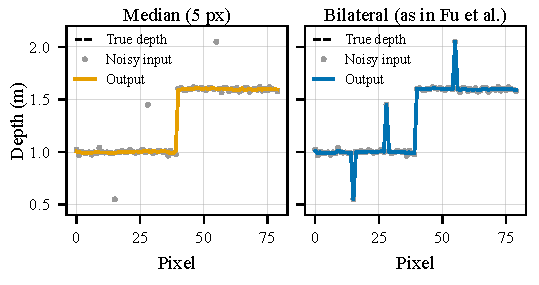
\includegraphics[width=\columnwidth]{fig2_filter_sketch.pdf}
\caption{A 1-D depth profile with a step edge and three spikes. The median
removes the spikes and keeps the edge. The bilateral filter, the core of
\fu{}, keeps the spikes, because a spike has no neighbour with a similar
depth to average with.}
\label{fig:sketch}
\end{figure}

\subsection{Method of \texorpdfstring{\fu{}}{Fu et al.}}

We re-implemented~\cite{fu2012kinect} in three steps.

\emph{1) Hole prediction.} Small holes are first filled with the mean of
their valid neighbours. Holes of 100 pixels or more are treated as out of
range and left empty. Then, for each pixel and each neighbouring frame
$t+i$ ($0<|i|\le2$), block matching finds the shift $\boldsymbol{\delta}_i$
(within $\pm6$ pixels) with the lowest mean squared error $\mathrm{MSE}_i$.
Each hole gets a weighted average of its matches (the sum over $i$ also
includes the $i=0$ term, discussed below):
\begin{equation}
\hat{D}_t(\mathbf{p}) =
\frac{\sum_{i} w_i\, D_{t+i}(\mathbf{p}+\boldsymbol{\delta}_i)}{\sum_{i} w_i},\qquad
w_i = e^{-\mathrm{MSE}_i^2/2\sigma_{\mathrm{mse}}^2}.
\label{eq:predict}
\end{equation}
The original divides by the number of frames instead of $\sum_i w_i$, which
would pull every prediction toward zero, so we normalise by the weights. The
paper is also unclear about the $i=0$ term, so we tried three readings
(include, exclude, search the current frame). They give the same results to
within 0.02\,cm, so we report only the first.

\emph{2) Spatio-temporal bilateral filter.} Each pixel becomes a weighted
average over $9\times9$ windows in frames $t-1$, $t$, $t+1$, centred at the
motion-compensated positions $\mathbf{p}+\boldsymbol{\delta}_j$, with
$\boldsymbol{\delta}_0=\mathbf{0}$ and $\boldsymbol{\delta}_{\pm1}$ from the
block matching:
\begin{multline}
D^\star_t(\mathbf{p}) = \frac{1}{W_\mathbf{p}}\sum_{j=-1}^{1}\;\sum_{\mathbf{q}\in S_{t+j}(\mathbf{p})}
G_s(\lVert\mathbf{p}+\boldsymbol{\delta}_j-\mathbf{q}\rVert)\\
\cdot G_r(\Delta)\, D_{t+j}(\mathbf{q}),
\label{eq:dnbl}
\end{multline}
where $S_{t+j}(\mathbf{p})$ is the window around
$\mathbf{p}+\boldsymbol{\delta}_j$, $\Delta=\hat{D}_t(\mathbf{p})-D_{t+j}(\mathbf{q})$,
$W_\mathbf{p}$ normalises the weights, $G_s$ is a Gaussian in pixel distance
($\sigma_s=2$\,px) and $G_r$ is a Gaussian in depth difference with standard
deviation $16\,\sigma_z$, where $\sigma_z = 2\,\mathrm{mm}\cdot z^2$ ($z$ in
metres) follows the quadratic Kinect noise
models~\cite{khoshelham2012accuracy,nguyen2012modeling}. At 1\,m the noise is
2\,mm and the kernel is 3.2\,cm wide. Parameters were tuned on ICL-NUIM frames 600 to 1400, which
do not overlap with the test frames.

\emph{3) What this means for spikes.} A spike differs from its neighbours by
far more than the width of $G_r$, so in~\eqref{eq:dnbl} only the spike itself
gets weight and it survives (Fig.~\ref{fig:sketch}). The method is built to
fill holes and smooth small noise, not to remove outliers.

\subsection{Depth-Only ICP Tracker}

Each depth map is turned into a point cloud. Consecutive frames are aligned
with ICP, coarse to fine on voxel grids of 4, 2 and 1\,cm, over
nearest-neighbour pairs closer than 10, 5 and 2\,cm. Pairs farther apart are
dropped, so large spikes usually have no partner and are ignored. Each frame
starts from the previous motion, and each level runs at most 30 iterations.

\emph{Point-to-point ICP (SVD).} This is the ICP of our proposal. For matched
pairs $(\mathbf{s}_k,\mathbf{d}_k)$, $k=1,\dots,N$, it seeks the rigid motion
$(\mathbf{R},\mathbf{t})$ that minimises
\begin{equation}
E_{\mathrm{pt}}(\mathbf{R},\mathbf{t}) = \sum_{k=1}^{N}
\bigl\lVert \mathbf{R}\mathbf{s}_k+\mathbf{t}-\mathbf{d}_k \bigr\rVert^{2},
\label{eq:p2p}
\end{equation}
which has a closed-form solution. Let $\boldsymbol{\mu}_s$ and
$\boldsymbol{\mu}_d$ be the mean points of the pairs, and take the singular
value decomposition
\begin{equation}
\mathbf{H}=\sum_{k=1}^{N}(\mathbf{s}_k-\boldsymbol{\mu}_s)
(\mathbf{d}_k-\boldsymbol{\mu}_d)^{\top}
=\mathbf{U}\boldsymbol{\Sigma}\mathbf{V}^{\top}.
\label{eq:svd}
\end{equation}
The optimal motion is
\begin{equation}
\mathbf{R}=\mathbf{V}\,\mathrm{diag}\bigl(1,1,\det(\mathbf{V}\mathbf{U}^{\top})\bigr)\,
\mathbf{U}^{\top},\qquad
\mathbf{t}=\boldsymbol{\mu}_d-\mathbf{R}\boldsymbol{\mu}_s,
\label{eq:rt}
\end{equation}
where the determinant factor keeps $\mathbf{R}$ a rotation and not a
reflection. Matching and solving alternate until the fit stops improving.

\emph{Point-to-plane ICP.} This variant counts only the distance along the
surface normal $\mathbf{n}_\mathbf{d}$ at the target point:
\begin{equation}
E(\mathbf{T}) = \sum_{(\mathbf{s},\mathbf{d})}
\bigl((\mathbf{T}\mathbf{s}-\mathbf{d})^{\top}\mathbf{n}_\mathbf{d}\bigr)^2 .
\label{eq:icp}
\end{equation}
Points may slide along a surface without cost, which usually converges faster
and more accurately~\cite{rusinkiewicz2001efficient}, but it needs good
normals. We run both variants and report the main results
(Table~\ref{tab:icp}) with point-to-plane, because it is more accurate in
every comparison (Table~\ref{tab:variants}). We also test point-to-plane with
a robust Tukey loss and GICP, all with the same settings.

% ===========================================================================
\section{Experimental Setup}

\emph{ICL-NUIM living room kt0}~\cite{handa2014benchmark}: synthetic, with
simulated Kinect noise, true depth and true camera path. Frames 1 to 300 are
used for depth error and every second frame (150 frames) for tracking. The
camera moves 6.5\,mm per tracked step, 0.97\,m in total. Holes: 0.84\%.

\emph{TUM RGB-D fr3/long\_office\_household}~\cite{sturm2012benchmark}: real
Asus Xtion data with a motion-capture path, no true depth. Every second frame
of frames 0 to 299 is tracked (150 frames). The camera moves 20.7\,mm per
step, 3.09\,m in total. Holes: 15.8\%.

\emph{Metrics.} Depth error is the mean absolute error (MAE) and RMS error
(RMSE) against the true depth. Since spikes are rare but large, they raise the
RMSE far more than the MAE, so RMSE\,$\gg$\,MAE means spikes are left.
Tracking error uses the two standard TUM metrics~\cite{sturm2012benchmark}.
The absolute trajectory error (ATE) is the RMS distance between estimated and
true camera positions after the best rigid alignment~\cite{horn1987closed}; it
measures total drift. The relative pose error (RPE) is the RMS error of each
single step; it measures local accuracy and does not accumulate.

% ===========================================================================
\section{Results}\label{sec:results}

\begin{figure}[!t]
\centering
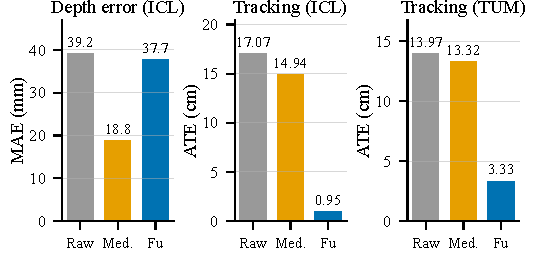
\includegraphics[width=\columnwidth]{fig3_key_result.pdf}
\caption{The main result (lower is better in all panels). By depth error the
median is the best denoiser and \fu{} is barely better than doing nothing. By
tracking error the order is reversed, on both datasets.}
\label{fig:key}
\end{figure}

\begin{table}[!t]
\caption{Depth Error on ICL-NUIM, Frames 1 to 300}
\label{tab:depth}
\centering
\small
\setlength{\tabcolsep}{2.5pt}
\begin{tabular}{@{}lcccc@{}}
\toprule
Method & MAE (mm) & RMSE (mm) & Within 1\,cm & Valid pixels\\
\midrule
No denoising & 39.2 & 187.5 & 42.2\% & 99.16\%\\
Median $9\times9$ & \textbf{18.8} & \textbf{55.4} & \textbf{44.7\%} & 99.16\%\\
\fu{}~\cite{fu2012kinect} & 37.7 & 186.0 & 33.7\% & \textbf{99.49\%}\\
\bottomrule
\end{tabular}
\end{table}

\begin{figure}[!t]
\centering
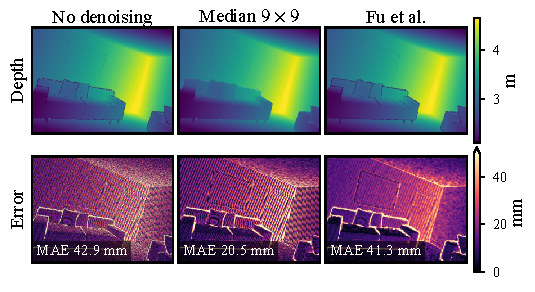
\includegraphics[width=\columnwidth]{fig4_depth_example.pdf}
\caption{ICL-NUIM frame 151. Top: denoised depth (holes white). Bottom: error
against the true depth, clipped at 50\,mm. The median clears the bright
speckle of spikes. \fu{} is smoother on flat areas but keeps the spikes.}
\label{fig:depth}
\end{figure}

Fig.~\ref{fig:key} summarises the paper. The rest of this section gives the
details.

\subsection{Depth Error: The Median Wins}

The input RMSE (187.5\,mm) is almost five times its MAE (39.2\,mm), so the
ICL-NUIM noise is mostly spikes (Table~\ref{tab:depth}). The median removes
them: it halves the MAE, cuts the RMSE by 3.4 times, and is better on every
one of the 300 frames (Fig.~\ref{fig:depth}). \fu{} barely changes the MAE and
leaves the RMSE at 186.0\,mm, because its bilateral filter keeps spikes
(Fig.~\ref{fig:sketch}). It does fill 40\% of the holes.

\begin{table}[!t]
\caption{Depth-Only Point-to-Plane ICP, 150 Frames. ATE (cm), Translational RPE (mm), Rotational RPE (deg)}
\label{tab:icp}
\centering
\small
\setlength{\tabcolsep}{3.5pt}
\begin{tabular}{@{}lcccccc@{}}
\toprule
& \multicolumn{3}{c}{ICL-NUIM kt0} & \multicolumn{3}{c}{TUM fr3 office}\\
\cmidrule(lr){2-4}\cmidrule(lr){5-7}
Depth used & ATE & RPE$_t$ & RPE$_r$ & ATE & RPE$_t$ & RPE$_r$\\
\midrule
\emph{True depth} & \emph{0.19} & \emph{0.07} & \emph{0.001} & n/a & n/a & n/a\\
No denoising & 17.07 & 14.43 & 0.426 & 13.97 & 11.69 & 0.476\\
Median $9\times9$ & 14.94 & 11.78 & 0.382 & 13.32 & 10.86 & 0.468\\
\fu{}~\cite{fu2012kinect} & \textbf{0.95} & \textbf{2.02} & \textbf{0.062} & \textbf{3.33} & \textbf{4.37} & \textbf{0.402}\\
\bottomrule
\end{tabular}
\end{table}

\begin{table}[!t]
\caption{ICP Variants: ATE (cm) / Translational RPE (mm). Bold: Best Variant per Row}
\label{tab:variants}
\centering
\small
\setlength{\tabcolsep}{3pt}
\begin{tabular}{@{}lccc@{}}
\toprule
Depth used & Point-to-point & Point-to-plane & Plane + Tukey\\
\midrule
\multicolumn{4}{@{}l}{\emph{ICL-NUIM kt0}}\\
True depth & 1.81 / 3.29 & 0.19 / 0.07 & \textbf{0.14 / 0.05}\\
No denoising & 36.96 / 21.36 & \textbf{17.05 / 14.38} & 22.47 / 17.47\\
Median $9\times9$ & 28.50 / 19.72 & \textbf{14.94 / 11.78} & 19.24 / 14.11\\
\fu{} & 1.93 / 3.16 & \textbf{0.95 / 2.02} & 1.42 / 2.54\\
\midrule
\multicolumn{4}{@{}l}{\emph{TUM fr3/long\_office\_household}}\\
No denoising & 27.24 / 14.92 & \textbf{13.97} / 11.69 & 14.31 / \textbf{11.55}\\
Median $9\times9$ & 18.14 / 13.78 & 13.33 / \textbf{10.86} & \textbf{13.07} / 10.96\\
\fu{} & 5.31 / 5.21 & 3.33 / 4.37 & \textbf{3.21 / 4.23}\\
\bottomrule
\end{tabular}
\end{table}

\begin{figure*}[!t]
\centering
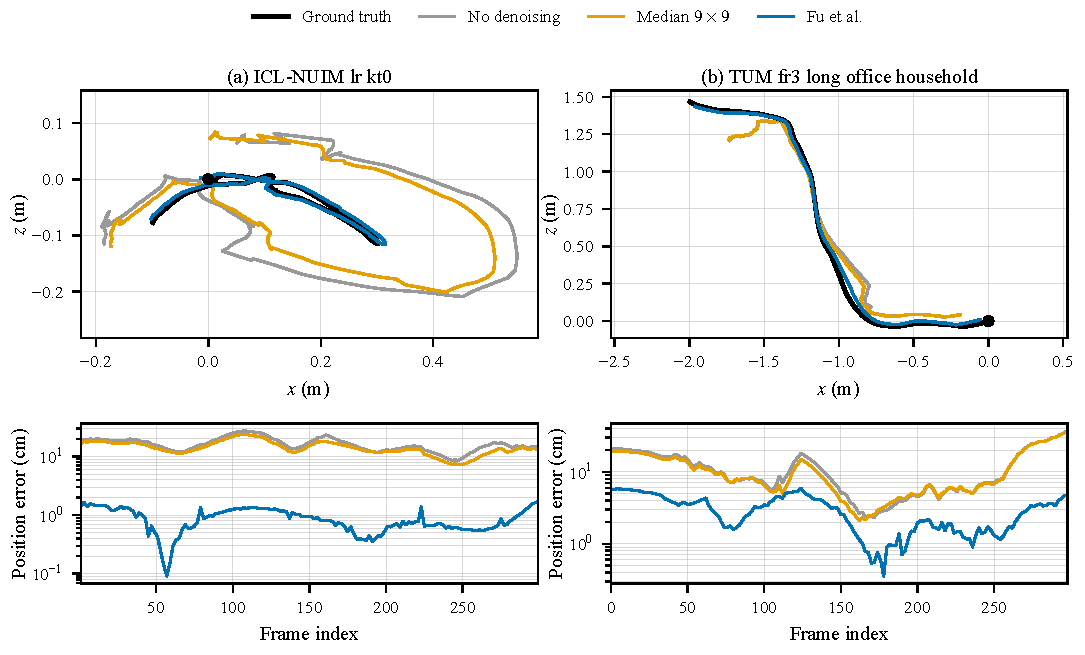
\includegraphics[width=0.96\textwidth]{fig5_camera_paths.pdf}
\caption{Estimated camera paths after alignment to the ground truth. Top: seen
from above. Bottom: position error per frame (log scale). (a) ICL-NUIM. (b) TUM
RGB-D. With the depth of \fu{} the path stays on the ground truth. With raw or
median-filtered depth it drifts by more than 10\,cm.}
\label{fig:paths}
\end{figure*}

\subsection{Tracking: \texorpdfstring{\fu{}}{Fu et al.} Wins by 4 to 16 Times}

Table~\ref{tab:icp} and Fig.~\ref{fig:paths} show the opposite ranking.
Compared with the median, \fu{} lowers the ATE 15.7 times on ICL-NUIM (0.95
vs.\ 14.94\,cm) and 4.0 times on TUM (3.33 vs.\ 13.32\,cm). The median is only
slightly better than no denoising at all. On ICL-NUIM its error per step
(11.78\,mm) is larger than the camera motion per step (6.5\,mm), so the
estimated motion is mostly noise. In short, \fu{} has twice the depth error of
the median but a 5.8 times smaller per-step tracking error.

\subsection{Other ICP Variants}

Is the result specific to point-to-plane ICP? Table~\ref{tab:variants} says
no. \fu{} beats the median under every variant that ran. Point-to-plane beats
point-to-point in all seven rows. The Tukey loss hurts on noisy ICL-NUIM depth
(it helps only on the true depth) and gives mixed results on TUM, where it
improves both errors only for the depth of \fu{}. GICP was unstable with our
untuned settings (it diverged on the median TUM depth and crashed on
ICL-NUIM), so we draw no conclusion about it. Small differences from
Table~\ref{tab:icp} (at most 0.02\,cm) come from a separate run.

\subsection{Filling the Holes Does Not Help}

Maybe the median loses because it leaves holes? We filled them with eight
methods (Table~\ref{tab:fill}), including the OpenCV~\cite{bradski2000opencv}
inpainting methods. On ICL-NUIM every fill is equal to or worse than keeping
the holes. The one gain, Navier-Stokes on TUM, does not repeat on ICL-NUIM.
Telea inpainting, the most common choice, is one of the least accurate
(87.0\,mm), because it blends the near and far sides of depth edges. Filled
depth is fine for display but should not be given to the tracker.

\begin{table}[!t]
\caption{Filling the Holes Left by the Median: Fill Error at Real ICL-NUIM Holes, ATE (cm) and Time per Frame (on TUM)}
\label{tab:fill}
\centering
\small
\setlength{\tabcolsep}{1.4pt}
\begin{tabular}{@{}lcccc@{}}
\toprule
Fill method & Error (mm) & ATE ICL & ATE TUM & Time\\
\midrule
None (keep holes) & n/a & \textbf{14.94} & 13.33 & 0\,ms\\
Telea~\cite{telea2004image} & 87.0 & 15.18 & 20.21 & 210\,ms\\
Navier-Stokes~\cite{bertalmio2001navier} & 22.5 & 15.36 & \textbf{12.03} & 224\,ms\\
Nearest valid pixel & 22.3 & 15.05 & 17.54 & 50\,ms\\
Region grow (small holes) & 15.5 & \textbf{14.94} & 13.32 & 52\,ms\\
Region grow (median) & 22.5 & 15.15 & 15.14 & 386\,ms\\
Background (far side) & 83.1 & 15.24 & 13.51 & 40\,ms\\
Temporal~\eqref{eq:predict} & \textbf{12.2} & 15.11 & 13.37 & 7.9\,s\\
\bottomrule
\end{tabular}
\end{table}

\subsection{Why the Median Does Not Help ICP}

Point-to-plane ICP~\eqref{eq:icp} needs two things: accurate normals
$\mathbf{n_d}$, and consecutive frames that describe the same surface. We
measured both on nine ICL-NUIM frames (Table~\ref{tab:normals}). For the
second, we moved frame $i+1$ onto frame $i$ using the \emph{true} motion and
measured the point-to-plane distance $e$. With perfect depth $e$ is close to
zero (0.3\,mm median, from sampling alone). A non-zero average of $e$ is a
bias that ICP will wrongly explain as camera motion.

\begin{table}[!t]
\caption{Normal Error and Frame-to-Frame Disagreement $e$ Under the True Motion (ICL-NUIM, 8 Frame Pairs)}
\label{tab:normals}
\centering
\small
\setlength{\tabcolsep}{4pt}
\begin{tabular}{@{}lccccc@{}}
\toprule
& \multicolumn{2}{c}{Normal error (deg)} & \multicolumn{3}{c}{Disagreement $e$ (mm)}\\
\cmidrule(lr){2-3}\cmidrule(lr){4-6}
Depth used & Median & Mean & $|e|$ median & Bias & RMS\\
\midrule
\emph{True depth} & n/a & n/a & \emph{0.3} & \emph{0.01} & \emph{1.1}\\
No denoising & 5.5 & 10.1 & 5.0 & 0.84 & 8.1\\
Median $9\times9$ & 2.8 & 7.4 & 3.6 & 1.09 & 6.4\\
\fu{} & \textbf{1.6} & \textbf{3.7} & \textbf{1.8} & \textbf{0.26} & \textbf{5.2}\\
\bottomrule
\end{tabular}
\end{table}

With \fu{}, the normal error is half that of the median, the frames agree
twice as well, and the bias is four times lower (0.26 vs.\ 1.09\,mm). The
median has the \emph{largest} bias of all, even larger than the raw depth.
This matches the tracking results: the median cleans each frame on its own, so
each frame is closer to the truth, but consecutive frames are cleaned
differently and no longer agree. \fu{} averages across frames, so its outputs
agree by design. The spikes it keeps cost little, because ICP drops point
pairs that are far apart.

% ===========================================================================
\section{Discussion}

\emph{Practical advice.} For depth-only tracking, use a denoiser that makes
consecutive frames consistent, such as \fu{}. For a single clean depth image,
the median is better, faster and simpler. If filled depth is needed for
display, use Navier-Stokes inpainting or the nearest valid pixel, not Telea,
and keep the filled pixels out of the tracker.

\emph{Cost.} The median handles 450 frames in under a minute. Our NumPy
version of \fu{} takes about 26 minutes, so it is not real-time as written.

\emph{Limitations.} We used one sequence per dataset, the normal analysis
covers only nine frames, and GICP was not tuned. Because \fu{} smooths over
both space and time, we cannot yet say which of the two matters more. Running
it with the temporal window set to zero would answer this. Adding colour
(RGB-D odometry) and more sequences are the next steps.

% ===========================================================================
\section{Conclusion}

A median filter halves the depth error of Kinect-style depth but barely
improves depth-only ICP tracking. The method of \fu{} leaves the depth error
almost unchanged but has 4 to 16 times less drift than the median (4 to 18
times less than no denoising). This holds for every ICP variant that ran and
is not changed by filling holes. The reason is that ICP compares frames with
each other: consistent, unbiased frames matter more than accurate individual
pixels. A depth denoiser should therefore be judged by the task it serves, not
by its per-pixel error.

\section*{Acknowledgment}

This work was carried out as a mini project for the course EE397 Design and
Development Task in Signal Processing at the National Institute of Technology
Karnataka, Surathkal. The authors thank Prof.~Krishnan CMC for the guidance
throughout the project.

\begin{thebibliography}{00}

\bibitem{newcombe2011kinectfusion}
R.~A. Newcombe \emph{et~al.}, ``KinectFusion: Real-time dense surface mapping
and tracking,'' in \emph{Proc. IEEE Int. Symp. Mixed and Augmented Reality
(ISMAR)}, 2011, pp.~127-136.

\bibitem{besl1992method}
P.~J. Besl and N.~D. McKay, ``A method for registration of 3-D shapes,''
\emph{IEEE Trans. Pattern Anal. Mach. Intell.}, vol.~14, no.~2, pp.~239-256,
Feb. 1992.

\bibitem{chen1992object}
Y.~Chen and G.~Medioni, ``Object modelling by registration of multiple range
images,'' \emph{Image Vis. Comput.}, vol.~10, no.~3, pp.~145-155, 1992.

\bibitem{fu2012kinect}
J.~Fu, S.~Wang, Y.~Lu, S.~Li, and W.~Zeng, ``Kinect-like depth denoising,'' in
\emph{Proc. IEEE Int. Symp. Circuits and Systems (ISCAS)}, 2012,
pp.~512-515.

\bibitem{huang1979fast}
T.~S. Huang, G.~J. Yang, and G.~Y. Tang, ``A fast two-dimensional median
filtering algorithm,'' \emph{IEEE Trans. Acoust., Speech, Signal Process.},
vol.~27, no.~1, pp.~13-18, Feb. 1979.

\bibitem{tomasi1998bilateral}
C.~Tomasi and R.~Manduchi, ``Bilateral filtering for gray and color images,''
in \emph{Proc. IEEE Int. Conf. Computer Vision (ICCV)}, 1998, pp.~839-846.

\bibitem{khoshelham2012accuracy}
K.~Khoshelham and S.~O. Elberink, ``Accuracy and resolution of Kinect depth
data for indoor mapping applications,'' \emph{Sensors}, vol.~12, no.~2,
pp.~1437-1454, 2012.

\bibitem{nguyen2012modeling}
C.~V. Nguyen, S.~Izadi, and D.~Lovell, ``Modeling Kinect sensor noise for
improved 3D reconstruction and tracking,'' in \emph{Proc. Int. Conf. 3D
Imaging, Modeling, Processing, Visualization and Transmission (3DIMPVT)},
2012, pp.~524-530.

\bibitem{rusinkiewicz2001efficient}
S.~Rusinkiewicz and M.~Levoy, ``Efficient variants of the ICP algorithm,'' in
\emph{Proc. Int. Conf. 3-D Digital Imaging and Modeling (3DIM)}, 2001,
pp.~145-152.

\bibitem{segal2009generalized}
A.~Segal, D.~Haehnel, and S.~Thrun, ``Generalized-ICP,'' in \emph{Proc.
Robotics: Science and Systems (RSS)}, 2009.

\bibitem{zhou2018open3d}
Q.-Y. Zhou, J.~Park, and V.~Koltun, ``Open3D: A modern library for 3D data
processing,'' arXiv:1801.09847, 2018.

\bibitem{handa2014benchmark}
A.~Handa, T.~Whelan, J.~McDonald, and A.~J. Davison, ``A benchmark for RGB-D
visual odometry, 3D reconstruction and SLAM,'' in \emph{Proc. IEEE Int. Conf.
Robotics and Automation (ICRA)}, 2014.

\bibitem{sturm2012benchmark}
J.~Sturm, N.~Engelhard, F.~Endres, W.~Burgard, and D.~Cremers, ``A benchmark
for the evaluation of RGB-D SLAM systems,'' in \emph{Proc. IEEE/RSJ Int. Conf.
Intelligent Robots and Systems (IROS)}, 2012, pp.~573-580.

\bibitem{horn1987closed}
B.~K.~P. Horn, ``Closed-form solution of absolute orientation using unit
quaternions,'' \emph{J. Opt. Soc. Amer. A}, vol.~4, no.~4, pp.~629-642, 1987.

\bibitem{telea2004image}
A.~Telea, ``An image inpainting technique based on the fast marching method,''
\emph{J. Graphics Tools}, vol.~9, no.~1, pp.~23-34, 2004.

\bibitem{bertalmio2001navier}
M.~Bertalm\'{i}o, A.~L. Bertozzi, and G.~Sapiro, ``Navier-Stokes, fluid
dynamics, and image and video inpainting,'' in \emph{Proc. IEEE Conf. Computer
Vision and Pattern Recognition (CVPR)}, 2001.

\bibitem{bradski2000opencv}
G.~Bradski, ``The OpenCV library,'' \emph{Dr. Dobb's Journal of Software
Tools}, 2000.

\end{thebibliography}

\end{document}
